%-------------------------------------------------------------------------------
\chapter{Chisel Basics}
\labelchapter{app.chisel}
    This Appendix provides motivations about technological choices that were made for this thesis, as well as some insights about basic usage of \chisel, the chosen \myLongAc{HCL}{Hardware Construction Language}.

    Doing so, we aim at providing more information about the usage of \myAcs{HCL} for hardware development.
    A particular focus is put on highlighting some notable differences with the standard \myLongAcs{HDL}{Hardware Description Language} such as \vhdl{} or \verilog{}, in order to help readers that may be familiar with such languages to comprehend the improvements that this paradigm enables.

    \section*{Motivation}
        \myLongAcs{HCL}{Hardware Construction Language} are a novel paradigm which enables the development of parametrized hardware generators instead of dedicated hardware accelerators, as described in Section \ref{ch.problem:sec.hardware:ssec.hcl}.
        Such initiatives are based on high level languages such as \python{} \cite{lockhart_pymtl_2014}, \haskell{} \cite{baaij_clash_2010} or \scala{} \cite{bachrach_chisel_2012}, which enable leveraging novel software constructs for hardware development.

        In this context, we chose to base this work on the usage of \myLongAc{Chisel}{Constructing Hardware in a Scala Embedded Language}, an \myAc{HCL} developed at Berkeley since 2012.
        Since its creation, \chisel{} has been widely adopted by both academic and industrial worlds, with initiatives such as the Rocket Chip generator \cite{asanovic_rocket_2016}, an in-order generator of RISC-V cores, the \myLongAc{BOOM}{Berkeley Out-of-Order Machine} generator \cite{celio_berkeley_2015}, an out-of-order version, or the development of Google \myLongAc{TPU}{Tensor Processing Unit} \cite{google_tpu_2018}.

        Moreover, Chisel has also been used as a basic tile of the Chipyard project \cite{chipyard_berkeley}, a set of tools used to create an agile framework for hardware development, along with tools such as Hammer \cite{wang_hammer_2018}, which decouples physical design concerns, logical design concerns, tool concerns and technology concerns, and Diplomacy \cite{cook_diplomatic_2017}, which enable automatic negotiation of parameters when generating complex Systems-on-a-Chip (SoC).
        It proves that Chisel ever growing community works to ever improve the language features, and that it can be used in wild, complex initiatives.

    \section*{Basic usage}
        To begin with, a simple cheat sheet is available in the project, in order to give some insights about available primitives for hardware generation \cite{chisel_cheatsheet_2021}.

        However, as an exhaustive comprehension of available constructs is not mandatory to understand the content of this work, examples of \chisel{} usage will be provided thereafter that should be sufficient to comprehend the improvements brought by \myAc{HCL} usage.

        \subsection*{Chisel compilation flow}
            The \chisel{} \myLongAc{HCF}{Hardware Construction Framework} structure is based on a separation of concerns inherited from the structure of software compilers, where the entry point ({\bf frontend}) and the tool output ({\bf backend}) are separated by an \myLongAc{IR}{Intermediate Representation}.
            Such architecture allows to implement support for various input and target languages, while exhibiting a modular structure for the developers.

            An example of a \chisel-based generation of a parametrized increment module is introduced in Figure \ref{app.chisel:fig.incr}, where two simple parameters are exhibited: the width of the module output, and its initialization value.

            Three main steps are taken during the generation of this module:
            \begin{enumerate}
                \item The \chisel{} parameters are resolved during the elaboration, meaning that the parameters are fixed for the remaining of the flow.
                    This is similar to the \verilog{} elaboration process where the explicit module parameters are resolved and propagated in the circuit description.

                    A {\bf high level} \firrtl{} representation is here generated as a first \myAc{IR}.
                \item Multiple transforms (including verifications such as combinatorial loop detection) are run over the \firrtl{} representation, progressively lowering the abstraction level, until a {\bf low level} representation is produced.

                    At the end of this process, all the data types and widths have been resolved, the conditional statements have been replaced, and it is guaranteed that every component is connected exactly once.\footnote{As the example module is very simple, no significant differences are exhibited between {\bf high} and {\bf low level} \firrtl{} representations.}

                    One can remark that, at this step, the parameters are fixed (\eg the width of the output is fixed to 8 bits) and implicit control signals --- \ie the clock and the reset --- have been generated automatically.
                \item The last step is a simple translation, where the {\bf low} \firrtl{} is translated to \verilog{}.

                    As the abstraction level remains the same, this process is quite straightforward, with the simple goal of providing an output language that can be used by most tools in the industry.
            \end{enumerate}

        \begin{figure}[h!]
            \centering
            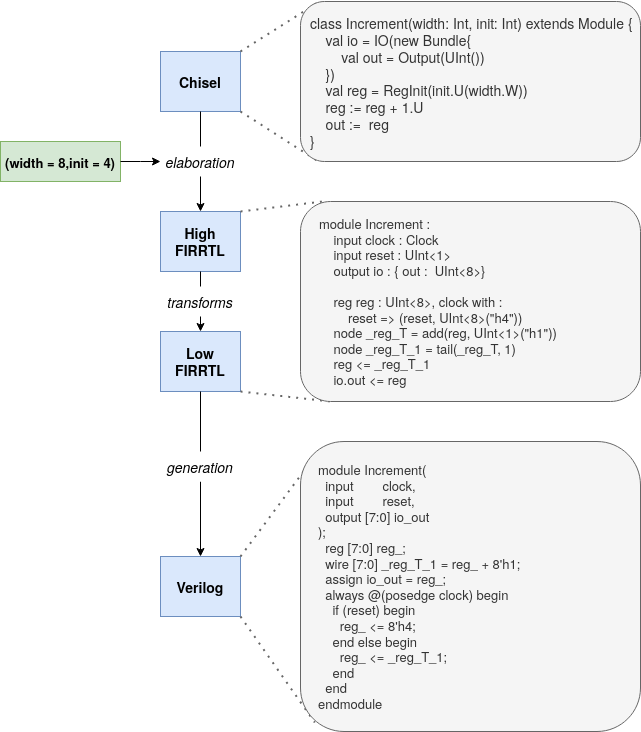
\includegraphics[width=1.0\textwidth]{Figures/flow-example}
            \caption{Implementing an increment module using \chiselT}
            \label{app.chisel:fig.incr}
        \end{figure}

        \subsection*{Exposing high level parameters at constructor level}
            One of the main differences of \myAcs{HCL} with standard \myAc{HDL} is the possibility to leverage \myLongAc{OOP}{Object-Oriented Programming} features --- such as module inheritance --- for hardware construction.
            While evolutions of those languages have come with a way to define simple \lstinline{parameter}s for module generation, as well as \lstinline{generate} features which enable loop based generation of hardware, it remains difficult to leverage complex parameters that could bring a lot for hardware generation.

            A simple example of a \chisel{} generator is introduced in Listing \ref{app.chisel:list.adder}, implementing a type parametric adder generator.
            It leverages a \scala{} constructor for module definition, allowing to define how each constructor parameter is used for adder generation --- meaning that the type of \lstinline{op1}, \lstinline{op2} and \lstinline{res} ports will be defined at elaboration time only. %\footnote{The process used to generate \verilog{} code from a \chisel{} {\bf Module} instance is called {\bf elaboration}. It consists in the iterative resolution of top level parameters, before running various \firrtl{} transforms in order to generate \myAc{RTL} code.}
            This code can then be used to generate variations of an adder module, allowing to instantiate an adder on 32 bit wide unsigned integers (line 14.) or on 8 bit fixed point numbers (line 15.) with the same description.

            Used parameter is here defined using the template feature from \scala, using a \lstinline{T} type for generation.
            This type is then checked at elaboration, to verify that it does implement the \lstinline{Data} type (the basic type for any data in \chisel) as well as the \lstinline{Num} trait (which ensure that a given type does implement basic arithmetic operations such as addition and multiplication).
            Doing so, one can leverage {\it polymorphism} to generate modules operating on any type that fits the requirements, enabling to build a library of easy to use components that can be adapted to multiple use cases.

            While this example is intentionally kept simple for the reader to understand the provided code, it should be noted that providing a similar module using standard \myAc{HDL} would require either to copy and adapt the code for every possible type, or search and replace type specific operations in the code.
            Moreover, more complex parameters can be defined, such as high-order functions which can be used as module parameters to change the behaviour of a circuit in functional fashion.

            \begin{figure}[h!]
                \begin{lstlisting}[numbers=left,stepnumber=1,
                                   caption={Type parametric adder generator in \chiselT},
                                   label={app.chisel:list.adder}]
import chisel3._
import chisel3.experimental.FixedPoint

class Adder[T <: Data with Num[T]](tpe: T)
    extends Module {
    val io = IO(new Bundle({
        val op1 = Input(tpe)
        val op2 = Input(tpe)
        val res = Output(tpe)
    })

    io.res := io.op1 + io.op2
}   

val uintAdder = new Adder(UInt(32.W))
val fpAdder = new Adder(FixedPoint(8.W, 3.BP))\end{lstlisting}
            \end{figure}

        \subsection*{Using functions as block generators}
            Another interesting feature of \chisel{} is the ability to generate hardware using functions to provide block abstractions --- in other terms, calling a function can result in \myAc{RTL} code generation at the end of the elaboration.

            \begin{figure}[h!]
                \vspace{-0.85cm}
                \begin{subfigure}{1.0\textwidth}
                    \begin{lstlisting}[language=Verilog,
                                       caption={Behavioural description of a register in Verilog},
                                       label={app.chisel:fig.register:list.verilog}]
module register (parameter WIDTH) (
    input clk,
    input reset,
    input [WIDTH-1:0] D,
    output [WIDTH-1:0] Q);

    reg [WIDTH-1:0] myregister;
    always @(posedge clk) begin
        if (reset)
            Q = 0;
        else
            Q = D;
endmodule\end{lstlisting}
                \end{subfigure}
                \begin{subfigure}{1.0\textwidth}
                    \begin{lstlisting}[caption={Building a register using \chiselT{} constructs},
                                       label={app.chisel:fig.register:list.chisel}]
class MyRegister[T: Data](tpe: T) extends Module {
    val io = IO(new Bundle{
        val dataIn = Input(tpe)
        val dataOut = Output(tpe)
    })
    // register width is inferred from dataIn type
    val myRegister = RegNext(dataIn)
    dataOut := myRegister
}\end{lstlisting}
                \end{subfigure}
                \caption{Building a register: HDL \vs{} HCL}
                \label{app.chisel:fig.register}
                \vspace{-0.55cm}
            \end{figure}

            This includes {\bf constructor methods}, meaning that the instantiation process can be leveraged to generate behavioural description of circuit.
            A simple example is provided in Figure \ref{app.chisel:fig.register}, where a \verilog{} description of a register (List. \ref{app.chisel:fig.register:list.verilog}) is compared to its \chisel{} counterpart (List. \ref{app.chisel:fig.register:list.chisel}).

            As can be observed here, the semantic for describing a register in standard \myAc{HDL} is based on simulation needs, as those languages were originally designed for simulation purposes instead of hardware description.
            One then needs to declare a logic signal (line 6.), and a process sensitive to the clock signal to either update the value, or reset it (lines 7-11).

            While every hardware developer has grown used to such way to describe registers, it remains a verbose way to describe a basic component that will be instantiated hundreds of times in a single circuit.
            Moreover, this semantic is quite confusing for beginners, as \verilog{} exposes a \lstinline[language=Verilog]{reg} keyword for signal declaration, but that does not actually differ from the \lstinline[language=Verilog]{wire} keyword from a semantic point of view.\footnote{The only way to describe a register is to use specific patterns such as the one in Listing \ref{app.chisel:fig.register:list.verilog}, that will be recognized and translated by synthesis tools to instantiate actual hardware registers.}

            On the other hand, \chisel{} leverages block generation through function calls, enabling users to simply instantiate basic classes for register description (line 6.).
            Once it is done, assigning a signal to the register value (\ie \lstinline{myRegister} value at line 6.) will change the next value (as does changing the value on port \lstinline{D} in List. \ref{app.chisel:fig.register:list.verilog}), while using the variable as a right-hand operand (line 7.) is equivalent to reading the content of the register (\lstinline{Q} port).

            This simple semantic is less error prone, as it does not rely on a copy of a particular pattern for instantiation, and allowing easier instantiation of basic component is a key feature to allow developers to spend more time on actual design problems, thus improving their productivity.
            We also see here that using high level parameters as exposed in previous section can enable to build highly reusable component generators, by defining a type parametric register module for example.

            \underline{Remark:} Both \lstinline{clk} and \lstinline{reset} signals are not provided for register instantiation in the \chisel{} example.
            In fact, those signals are implicit in any class inheriting from \lstinline{Module}, the basic class for hardware circuits.
            They are used for instantiations of components that require them, and are being propagated to every instantiated sub module in order to expose coherent time zones to users.
            If needed, they can be overwritten manually to build different time zones --- \eg for circuits using multiple clock domains.

        \subsection*{Leveraging high level constructs for generation}
            The last feature that we will consider here is the usage of high level functionalities for hardware generation.

            As \chisel{} is based on \scala{} language, features from this language can be used to define module generators and bring more expressivity for developers.

            \begin{figure}[h!]
                \begin{lstlisting}[caption={Building a dot product kernel using \chiselT},
                                   label={app.chisel:list.mac}]
class DotProduct(width: Int, nElem: Int) extends Module {
    val dataType = UInt(width.W)

    val io = IO(new Bundle{
        val op1 = Input(Vec(nElem, dataType))
        val op2 = Input(Vec(nElem, dataType))
        val out = Output(dataType)
    })

    io.out := ((io.op1 zip io.op2)
        .map{ case (a, b) => a * b })
        .reduceTree(_ + _) // use balanced tree
}\end{lstlisting}
            \end{figure}

            Listing \ref{app.chisel:list.mac} introduces a {\bf dot product} generator parametrized by elements width and number.
            This generator thus accepts two vectors of elements, which elements are multiplied two by two, before being summed to produce the output.
            Such operation can be captured using the {\bf map-reduce} paradigm, as it would be done in a software implementation leveraging functional programming, and hardware designers should also benefit from such programming patterns.

            An example of the target architecture is provided in Figure \ref{app.chisel:fig.dot}, to help the reader to understand the gap between the final circuit, and what the designer actually requires to describe using either \chisel{} or \verilog.

            Lines 9. to 11. expose how \chisel{} can be leveraged to build a generator for such implementations: input vectors are {\bf zipped} --- \ie elements of each vectors are paired --- before multiplication is applied to each pair.
            Resulting vector is then reduced through add operations, using a binary tree structure to force elaboration to produce a balanced adder tree.

            \begin{figure}[h!]
                \begin{lstlisting}[language=Verilog,basewidth={0.5em, 0.4em},tabsize=2,numbers=none,xleftmargin=-2mm,
                                   caption={Dot product generic implementation in Verilog},
                                   label={app.chisel:list.verilogDP}]
module dot_product #(
    parameter NELEM,
    parameter WIDTH,
  ) (
    input [N-1:0] [WIDTH-1:0] op1,
    input [N-1:0] [WIDTH-1:0] op2,
    output        [WIDTH-1:0] out,
  );

  localparam  STAGES = clog2(NELEM);
  localparam  NPADDED = 2**(STAGES);

  wire  [STAGES:0] [NPADDED-1:0] [WIDTH-1:0] tab;

  generate
    // Init loop with mul (required padding for NELEM not power of 2)
    for (i=0; i<NPADDED; i=i+1) begin:init
      // 0 padding is fine for add reduce
      assign tab[0][i] = (i < NELEM) ? op1[i] * op2[i] : '0;
    end

    // main reduce loop with tree
    for (stage=0; stage<STAGES; stage=stage+1) begin:stages
      for (couple=0; couple<2**(STAGES-stage-1); couple=couple+1)
        begin:couples
          localparam first  = couple * (2**(stage+1));
          localparam second = first + (2**stage);
          assign tab[stage+1][first] =
            tab[stage][first] + tab[stage][second];
      end
    end
  endgenerate

  assign out = tab[STAGES][0];
endmodule\end{lstlisting}
            \end{figure}

            A \verilog{} counterpart is proposed in Listing \ref{app.chisel:list.verilogDP}, to exhibit the complexity of building such generator in a traditional \myAc{HDL}.
            To do so, we require to expose a multidimensional array of elements and populate it according to some specific patterns on the indexes, through the \lstinline[language=Verilog]{generate ... for} construct.
            This pattern is hence recognized by the synthesis tool, which eliminates the useless elements of the array, and build the correct adder tree.

\clearpage
            A last remark can be done on the differences between those two paradigms: while changing the data path of the \verilog{} module --- \eg to add registers after multipliers and adders --- requires to modify the whole code, it can be done in a functional way in the \chisel{} description.

            This is possible because both \lstinline{map} and \lstinline{reduceTree} functions accept high-order functions as parameters to define which operations are to be performed, which is known in the software world as {\bf functional programming}.
            In fact, the \lstinline{reduceTree} construct even accepts a second function as parameter, to define what to do on non balanced trees (when the number of elements is not a power of two), allowing to define a simple delay using a \lstinline{RegNext} in the case of pipelined additions, for instance.

            This final example thus exhibits how the introduced features enable to build efficient hardware generators which are easier to design, understand and adapt to new use cases.

            \begin{figure}[h!]
                \centering
                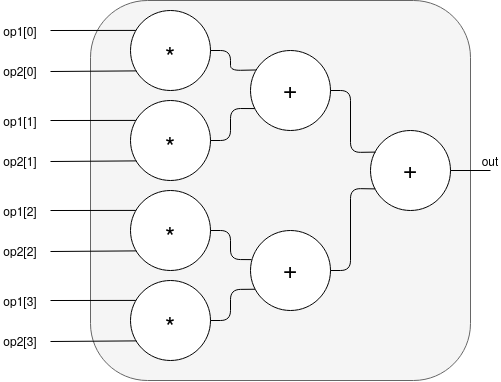
\includegraphics[width=1.0\textwidth]{Figures/dot-archi}
                \caption[Example of a dot product architecture to generate]{Example of a dot product architecture to generate\newline ({\it using vectors of 4 elements})}
                \label{app.chisel:fig.dot}
            \end{figure}
            

